\documentclass{article}
\usepackage{arxiv}

% Компиляция: pdfLaTeX (Overleaf) или XeLaTeX — преамбула работает с обоими.
\usepackage{iftex}
\ifPDFTeX
  \usepackage[T2A]{fontenc}
  \usepackage[utf8]{inputenc}
\else
  \usepackage{fontspec}
  \setmainfont{Liberation Serif}
  \setsansfont{DejaVu Sans}
  \setmonofont{DejaVu Sans Mono}
  \newfontfamily\cyrillicfont{Liberation Serif}
  \newfontfamily\cyrillicfontsf{DejaVu Sans}
  \newfontfamily\cyrillicfonttt{DejaVu Sans Mono}
\fi
\ifPDFTeX
  \usepackage[english, russian]{babel}
\else
  \usepackage{polyglossia}
  \setdefaultlanguage{russian}
  \setotherlanguage{english}
\fi
\usepackage{url}
\usepackage{booktabs}
\usepackage{amsmath, amssymb, amsfonts, amsthm}
\usepackage{nicefrac}
\usepackage{microtype}
\usepackage{graphicx}
\usepackage[numbers, sort&compress]{natbib}
\usepackage{doi}
\usepackage{xcolor}
\usepackage{algorithm}
\usepackage{algpseudocode}
\usepackage{tabularx}

\newtheorem{assumption}{Гипотеза}
\newtheorem{theorem}{Теорема}
\newtheorem{corollary}{Следствие}
\theoremstyle{definition}
\newtheorem{definition}{Определение}
\theoremstyle{remark}
\newtheorem{remark}{Замечание}

\floatname{algorithm}{Алгоритм}
\renewcommand{\algorithmicrequire}{\textbf{Вход:}}
\renewcommand{\algorithmicensure}{\textbf{Выход:}}

% Места, где числа появятся после пересчёта реальных данных
\newcommand{\todo}[1]{\textcolor{red}{[#1]}}

\newcommand{\R}{\mathbb{R}}
\newcommand{\E}{\mathbb{E}}
\newcommand{\Var}{\operatorname{Var}}
\newcommand{\tr}{\operatorname{tr}}
\newcommand{\bx}{\mathbf{x}}
\newcommand{\be}{\mathbf{e}}
\newcommand{\bone}{\mathbf{1}}
\newcommand{\Lbar}{\bar{L}}
\newcommand{\Ibar}{\bar{I}}
\newcommand{\aBT}{a_{\mathrm{BT}}}
\newcommand{\aH}{a_{\mathrm{H}}}
\newcommand{\mBT}{m_{\mathrm{BT}}}

\title{Сколько попарных сравнений заменяют признаки объектов: априорный прогноз для иерархической модели Брэдли--Терри}

% TODO: вписать ФИО автора и научного руководителя
\author{И.~О.~Фамилия \\
	Факультет ВМК МГУ имени М.~В.~Ломоносова\\
	\And
	Научный руководитель: И.~О.~Фамилия \\
}
\date{}

\renewcommand{\shorttitle}{Признаки заменяют часть попарного опроса}

\hypersetup{
pdftitle={Сколько попарных сравнений заменяют признаки объектов},
pdfkeywords={модель Брэдли--Терри, попарные сравнения, планирование опроса, лапласово приближение, малоресурсные языки},
}

\begin{document}
\maketitle

\begin{abstract}
Статья посвящена планированию опросов, в которых люди попарно сравнивают объекты, например варианты замены заимствованного слова. Такие опросы дороги, особенно для малоресурсных языков, носителей которых трудно привлечь. Цель работы~--- до сбора данных предсказать, во сколько раз признаки объектов сокращают число сравнений, нужное для заданного качества ранжирования. Рассматривается иерархическая модель Брэдли--Терри, в которой полезность объекта есть сумма линейной функции признаков и индивидуального отклонения. В лапласовом приближении получена замкнутая формула экономии через долю дисперсии предпочтений, объясняемую признаками. Для произвольного плана опроса доказаны спектральные границы экономии и показано, что формула со средней информацией сравнения даёт нижнюю оценку ожидаемого риска. Предложен уточнённый априорный прогноз методом Монте-Карло, учитывающий случайность плана и неравную информативность пар. В вычислительном эксперименте уточнённый прогноз совпадает с измеренной экономией в пределах 5\,\% во всех рассмотренных режимах, а разреженные планы опроса дают до двух раз большую экономию, чем случайный выбор пар. Метод проверен на открытых данных, где носители английского языка как иностранного оценивали сложность слов\todo{: итог по реальным данным после пересчёта}. Полученные результаты позволяют рассчитать объём опроса носителей до его проведения.
\end{abstract}

\keywords{модель Брэдли--Терри \and попарные сравнения \and планирование опроса \and лапласово приближение \and малоресурсные языки}

%=====================================================================
\section{Введение}

Многие решения в обработке языка опираются на суждения людей, а не на автоматические метрики. Так устроена задача, послужившая отправной точкой работы: для русского заимствования в татарском языке нужно выбрать лучшую из нескольких замен, предложенных словообразовательными правилами или языковой моделью. Мерилом здесь служит мнение носителей, а носителей малоресурсного языка трудно и дорого привлечь к опросу~\citep{joshi2020state}. Поэтому главный вопрос планирования~--- сколько ответов людей понадобится для надёжного ранжирования и сколько из них можно заменить знанием о самих объектах.

Назовём \emph{объектом} кандидата на замену, \emph{группой}~--- набор кандидатов для одного заимствования, \emph{сравнением}~--- ответ человека на вопрос, какой из двух кандидатов внутри группы лучше. Классическая модель Брэдли--Терри~\citep{bradley1952rank, luce1959individual} приписывает каждому объекту скрытую полезность $u_i$ и считает вероятность выбора $i$ в паре $(i,j)$ равной $\sigma(u_i-u_j)$. \emph{Признаки} объекта~--- измеримые свойства слова (частота, длина, правдоподобие формы для языка), которые могут частично объяснять полезность. Основная идея работы: если признаки объясняют долю $\rho$ разброса полезностей, то часть информации, которую иначе пришлось бы собирать сравнениями, известна заранее, и эту часть можно выразить в числе сравнений.

Модели предпочтений с признаками известны давно~\citep{springall1973response, turner2012bradleyterry2} и в байесовской форме совпадают с обучением предпочтениям на гауссовских процессах~\citep{chu2005preference, houlsby2012collaborative}; нейросетевой вариант той же идеи лежит в основе моделей вознаграждения при обучении языковых моделей по отзывам людей~\citep{christiano2017deep, ouyang2022training}. Сколько сравнений нужно без признаков, изучено подробно: погрешность оценок определяется спектром лапласиана графа сравнений~\citep{shah2016estimation, hajek2014minimax} или его эффективным сопротивлением~\citep{hendrickx2019graph}, а адаптивный выбор пар сокращает опрос~\citep{jamieson2011active, heckel2019active, maystre2017just}. Отдельное направление объединяет немного ответов людей с большим числом предсказаний модели так, чтобы выводы оставались несмещёнными~\citep{angelopoulos2023prediction, chatzi2024prediction, boyeau2025autoeval}.

Эти работы оставляют открытым практический вопрос планирования: \emph{во сколько раз} априорная информация о полезностях сокращает опрос при заданном плане и как это предсказать \emph{до} сбора данных. Минимаксные оценки~\citep{shah2016estimation} не учитывают признаков; работы о гауссовских процессах~\citep{chu2005preference} предлагают модель, но не формулу объёма опроса; методы, основанные на предсказаниях~\citep{angelopoulos2023prediction}, гарантируют несмещённость, но не дают простого правила пересчёта признаков в число сравнений. Понятие эффективного размера выборки априорного распределения~\citep{morita2008determining} близко по смыслу, но не применялось к моделям попарных сравнений и к выбору плана опроса.

В работе предлагается априорный прогноз экономии сравнений для иерархической модели Брэдли--Терри $u_i=\theta^{\top}\bx_i+\eta_i$. Он получен в лапласовом приближении~\citep{tierney1986accurate} и зависит только от доли $\rho$, разброса полезностей, размера групп и плана опроса. Вклад работы:
\begin{enumerate}
	\item замкнутая формула экономии~\eqref{eq:closed} для случайного выбора пар внутри групп;
	\item спектральные границы экономии для произвольного плана (теорема~\ref{thm:bounds}) и следствие: признаки ценнее всего при разреженном опросе;
	\item доказательство того, что формула со средней информацией сравнения даёт нижнюю оценку ожидаемого риска (теорема~\ref{thm:jensen}), и уточнённый прогноз методом Монте-Карло, совпадающий с экспериментом в пределах 5\,\%;
	\item проверка на синтетических данных и на открытых человеческих оценках сложности английских слов~\citep{maddela2018word, paetzold2016benchmarking}, где структура данных повторяет задачу выбора замены.
\end{enumerate}

Цель вычислительного эксперимента~--- проверить, что прогноз до эксперимента совпадает с измеренной экономией, выяснить, какие допущения теории ответственны за расхождения, и оценить, переносится ли вывод на реальные человеческие сравнения. Код и данные эксперимента открыты\footnote{\todo{ссылка на репозиторий проекта на GitHub}}.

\begin{table}[t]
\caption{Близкие подходы к ранжированию по попарным сравнениям. Ни один из них не даёт априорной формулы, переводящей информацию признаков в число сравнений при заданном плане опроса.}
\label{tab:related}
\centering\small
\begin{tabularx}{\linewidth}{>{\raggedright\arraybackslash}p{3.6cm} >{\raggedright\arraybackslash}X >{\raggedright\arraybackslash}X}
\toprule
Подход & Сильные стороны & Слабые стороны \\
\midrule
Брэдли--Терри без признаков~\citep{bradley1952rank, hunter2004mm} & простота, состоятельность, быстрые алгоритмы & нужно много сравнений на каждый объект; новые объекты без истории не оцениваются \\
Только признаки, модели вознаграждения~\citep{springall1973response, christiano2017deep, ouyang2022training} & обобщение на новые объекты & ошибка признаков не исправляется сравнениями этого объекта \\
Гауссовские процессы, байесовская BT~\citep{chu2005preference, houlsby2012collaborative, caron2012efficient} & объединяют признаки и сравнения & нет правила для объёма опроса \\
Минимаксные границы и топология графа~\citep{shah2016estimation, hendrickx2019graph} & точные оценки числа сравнений и роль плана & не учитывают априорную информацию \\
Активный выбор пар, дуэльные бандиты~\citep{jamieson2011active, heckel2019active, bengs2021preference} & меньше сравнений за счёт адаптивности & требуют онлайн-опроса; не используют признаки \\
Вывод на основе предсказаний~\citep{angelopoulos2023prediction, chatzi2024prediction} & несмещённость при ошибочных предсказаниях & выигрыш ограничен корреляцией предсказаний с людьми \\
\midrule
Данная работа & априорный прогноз экономии для любого плана; границы и нижняя оценка риска & гауссовское приближение; признаки линейны \\
\bottomrule
\end{tabularx}
\end{table}

%=====================================================================
\section{Обзор литературы}
\label{sec:review}

\paragraph{Модели попарных сравнений.}
Модель Терстоуна~\citep{thurstone1927law} и модель Брэдли--Терри--Льюса~\citep{bradley1952rank, luce1959individual} описывают выбор в паре через разность скрытых полезностей; они отличаются лишь функцией связи (нормальной или логистической). Оценка максимального правдоподобия для обобщённых моделей Брэдли--Терри вычисляется MM-алгоритмами~\citep{hunter2004mm}, обзор моделей, в том числе для зависимых данных, дан в~\citep{cattelan2012models}. Агрегирование сравнений, собранных краудсорсингом, требует учёта качества исполнителей~\citep{chen2013pairwise, dawid1979maximum, snow2008cheap}; сравнительные шкалы при этом надёжнее оценок по шкале Ликерта~\citep{kiritchenko2017best}. Нам эти работы дают модель и базовый метод~--- модель Брэдли--Терри без признаков.

\paragraph{Признаки и априорная информация.}
Зависимость полезности от признаков объекта вводилась в модель Брэдли--Терри ещё в~\citep{springall1973response} и реализована в пакете~\citep{turner2012bradleyterry2}, где к линейной части добавляется случайный эффект объекта~--- это и есть иерархическая модель настоящей работы. Байесовская трактовка с гауссовским процессом в качестве априорного распределения предложена в~\citep{chu2005preference} и развита для многих пользователей в~\citep{houlsby2012collaborative}; рейтинговые системы вроде TrueSkill~\citep{herbrich2007trueskill} используют ту же схему с последовательным обновлением, а точный байесовский вывод для моделей Брэдли--Терри построен в~\citep{caron2012efficient}. Модели вознаграждения в обучении по отзывам людей~\citep{christiano2017deep, ouyang2022training}~--- предельный случай <<только признаки>> с нейросетевой функцией признаков. Во всех этих работах признаки служат для лучшего предсказания, но не ставится вопрос, сколько ответов людей они заменяют. Ближе всего к нему понятие эффективного размера выборки априорного распределения~\citep{morita2008determining}; мы конкретизируем его для попарных сравнений и связываем с планом опроса.

\paragraph{Сколько сравнений нужно.}
Минимаксные границы ошибки оценивания в модели Брэдли--Терри выражаются через спектр лапласиана графа сравнений~\citep{shah2016estimation, hajek2014minimax}; спектральные алгоритмы и регуляризованное максимальное правдоподобие оптимальны для выбора лучших $K$ объектов~\citep{negahban2017rank, chen2015spectral, chen2019spectral}, а для непараметрических моделей достаточно подсчёта побед~\citep{shah2018simple}. Связь ошибки с эффективным сопротивлением графа позволяет выбирать план опроса без адаптивности~\citep{hendrickx2019graph}, асимптотические доверительные интервалы получены в~\citep{gao2023uncertainty}. Эти результаты описывают модель без априорной информации; наша теорема~\ref{thm:bounds} показывает, как добавление априорной точности сдвигает спектр и почему выигрыш больше на разреженных графах.

\paragraph{Выбор пар.}
Активное ранжирование сокращает число сравнений, если пары выбираются по ходу опроса~\citep{jamieson2011active, heckel2019active, maystre2017just}; задача поиска лучшего объекта по сравнениям изучается как дуэльные бандиты~\citep{yue2012karmed, bengs2021preference}, а байесовское планирование эксперимента~\citep{chaloner1995bayesian, houlsby2011bayesian} выбирает наиболее информативные вопросы. Адаптивность требует онлайн-опроса, тогда как опрос носителей часто проводится статичной анкетой; наш прогноз относится именно к плану, зафиксированному заранее.

\paragraph{Ответы людей и предсказания моделей.}
Вывод на основе предсказаний (prediction-powered inference) объединяет небольшую размеченную выборку с предсказаниями модели и сохраняет корректность доверительных интервалов~\citep{angelopoulos2023prediction, angelopoulos2023ppipp}; этот подход применён к оценке моделей~\citep{boyeau2025autoeval}, к ранжированию языковых моделей по попарным сравнениям~\citep{chatzi2024prediction} и к активному выбору объектов для разметки~\citep{zrnic2024active}. Языковые модели всё чаще используются как судьи~\citep{zheng2023judging, chiang2024chatbot} и аннотаторы~\citep{gilardi2023chatgpt}, но для неанглийских языков их оценки требуют калибровки по носителям~\citep{hada2024large}. В нашей постановке предсказание модели~--- ещё один вид признака; выигрыш выражается не в ширине интервала, а в числе сравнений.

\paragraph{Прикладной контекст.}
Задача выбора замены слова по суждениям людей изучается в лексическом упрощении: для целевого слова собираются кандидаты и упорядочиваются по простоте~\citep{specia2012semeval, paetzold2016benchmarking, paetzold2017survey, qiang2020lexical, saggion2022findings}; сложность слов оценивается людьми по шкале~\citep{maddela2018word, shardlow2020complex}. Правдоподобие новой формы для носителей связано с фонотактикой и лексическим окружением~\citep{bailey2001determinants, hayes2008maximum}, а появление неологизмов~--- с распределением смыслов~\citep{ryskina2020where}. Для татарского языка доступны морфологические анализаторы~\citep{washington2014finite} и тесты понимания языка~\citep{isbarov2025tumlu}, но нет данных о предпочтениях носителей между заменами заимствований~\citep{haspelmath2009loanwords}. Поэтому данные лексического упрощения служат в работе проверочным полигоном с той же структурой.

\paragraph{Вывод.}
Существующие работы дают модель с признаками, оценки числа сравнений без признаков и способы объединять людей с предсказаниями, но не дают априорного правила: сколько сравнений заменяют признаки при заданном плане опроса. Построению такого правила и проверке его точности посвящена работа.

%=====================================================================
\section{Постановка задачи}
\label{sec:problem}

\paragraph{Общее описание.}
Дано несколько групп объектов (замены для каждого заимствования) с признаками. Люди сравнивают объекты попарно внутри групп по заранее выбранному плану. Требуется упорядочить объекты в каждой группе по предпочтениям людей и до сбора данных предсказать, во сколько раз использование признаков сокращает число сравнений, необходимых для заданного качества.

\paragraph{Данные.}
Множество объектов $\{1,\dots,N\}$ разбито на $G$ групп $S_1,\dots,S_G$, $|S_g|=K$, $N=GK$. Объекту $i$ сопоставлен вектор признаков $\bx_i\in\R^d$, матрица признаков $X\in\R^{N\times d}$. План опроса~--- распределение $q=(q_e)$ на парах $e=\{i,j\}$ внутри групп. Выборка $\mathcal D_m=\{(w_t,l_t)\}_{t=1}^{n}$ из $n=\lfloor mN/2\rceil$ сравнений: пара выбирается по плану $q$, $w_t$~--- выбранный человеком объект, $l_t$~--- второй. Параметр $m$ (\emph{бюджет})~--- среднее число сравнений на объект.

\begin{assumption}[модель выбора]\label{as:bt}
Существует вектор полезностей $u\in\R^N$, при фиксированных парах исходы сравнений независимы и $P(i\succ j)=\sigma(u_i-u_j)$, $\sigma(z)=1/(1+e^{-z})$.
\end{assumption}

\begin{assumption}[порождение полезностей]\label{as:hier}
$u_i=\theta^{\top}\bx_i+\eta_i$, где $\eta_i\sim\mathcal N(0,\sigma_\eta^2)$ независимы между собой и с $\bx_i$. Обозначим $V=\Var(u_i)$ и долю дисперсии, объясняемую признаками,
\begin{equation}\label{eq:rho}
\rho=\frac{\Var(\theta^{\top}\bx_i)}{\Var(u_i)}, \qquad \sigma_\eta^2=(1-\rho)V.
\end{equation}
\end{assumption}

\paragraph{Модели.}
Оценка полезностей $s=X\theta+\eta$ (иерархическая модель, предлагаемая); частные случаи~--- модель Брэдли--Терри без признаков ($\theta=0$, базовый метод) и модель <<только признаки>> ($\eta=0$, второй базовый метод).

\paragraph{Внутренний критерий.}
Штрафованное отрицательное логарифмическое правдоподобие (MAP-оценка при гауссовских априорных распределениях):
\begin{equation}\label{eq:criterion}
(\hat\theta,\hat\eta)=\arg\min_{\theta,\eta}\; Q(\theta,\eta),\quad
Q=-\sum_{t=1}^{n}\log\sigma\bigl(s_{w_t}-s_{l_t}\bigr)+\frac{\lambda}{2}\|\eta\|^2+\frac{\lambda_\theta}{2}\|\theta\|^2 .
\end{equation}
Параметр $\lambda$ выбирается из сетки $\Lambda$ по правдоподобию отложенных сравнений (в синтетике~--- 20\,\% случайных сравнений, на реальных данных~--- все сравнения одного аннотатора), $\lambda_\theta=10^{-2}$.

\paragraph{Внешние критерии.}
Качество ранжирования~--- среднее по группам значение $\tau$ Кендалла между оценками $s$ и истинными полезностями $u$:
\begin{equation}\label{eq:tau}
\bar\tau(s)=\frac1G\sum_{g=1}^{G}\tau\bigl(s_{S_g},u_{S_g}\bigr).
\end{equation}
Дополнительно: доля групп, где лучший по оценке объект совпадает с лучшим по эталону (top-1); среднее отрицательное логарифмическое правдоподобие контрольных сравнений; среднеквадратичная ошибка внутригрупповых контрастов
\begin{equation}\label{eq:mse}
\mathrm{MSE}(s)=\frac1N\sum_{g=1}^{G}\sum_{i\in S_g}\bigl((s_i-\bar s_g)-(u_i-\bar u_g)\bigr)^2,
\end{equation}
где $\bar s_g$, $\bar u_g$~--- средние по группе (ранжирование внутри группы не зависит от сдвига группы целиком).

\paragraph{Исследуемая величина.}
Пусть $\mathcal Q_M(m)$~--- ожидаемое значение внешнего критерия для метода $M$ при бюджете $m$. \emph{Эквивалентный бюджет} модели без признаков и \emph{экономия} при бюджете $m_0$ иерархической модели:
\begin{equation}\label{eq:saving}
\mBT(m_0)=\min\bigl\{m:\ \mathcal Q_{\mathrm{BT}}(m)\ge \mathcal Q_{\mathrm H}(m_0)\bigr\},\qquad
\kappa(m_0)=\frac{\mBT(m_0)}{m_0}.
\end{equation}
Для MSE неравенство обращается. \textbf{Задача:} построить прогноз $\hat\kappa(m_0;\rho,V,K,q)$, вычислимый до сбора данных, и оценить его точность.

%=====================================================================
\section{Метод и теоретические свойства}
\label{sec:method}

\subsection{Алгоритм обучения}

Критерий~\eqref{eq:criterion} гладкий и выпуклый по $(\theta,\eta)$ (сумма выпуклых функций $-\log\sigma$ от линейных форм и положительно определённых квадратичных штрафов), поэтому минимум единственен и находится квазиньютоновским методом L-BFGS. Градиент вычисляется за $O(n+Nd)$ операций.

\begin{algorithm}[h]
\caption{Иерархическая модель Брэдли--Терри}\label{alg:fit}
\begin{algorithmic}[1]
\Require матрица признаков $X$, сравнения $\mathcal D$, сетка $\Lambda$, $\lambda_\theta$, правило отложенной выборки
\Ensure оценки полезностей $s=X\hat\theta+\hat\eta$
\State разбить $\mathcal D$ на обучающую $\mathcal D_{\mathrm{tr}}$ и отложенную $\mathcal D_{\mathrm{val}}$ части
\For{$\lambda\in\Lambda$}
	\State $(\theta_\lambda,\eta_\lambda)\gets\arg\min Q$ на $\mathcal D_{\mathrm{tr}}$ (L-BFGS из нуля)
	\State $\ell(\lambda)\gets$ среднее $-\log\sigma(s_w-s_l)$ на $\mathcal D_{\mathrm{val}}$
\EndFor
\State $\lambda^*\gets\arg\min_\lambda \ell(\lambda)$; $(\hat\theta,\hat\eta)\gets\arg\min Q$ на всём $\mathcal D$ при $\lambda^*$
\end{algorithmic}
\end{algorithm}

\subsection{Риск в лапласовом приближении}

Чтобы получить прогноз до сбора данных, рассмотрим идеализированный случай: среднее $\mu_i=\theta^{\top}\bx_i$ известно (\emph{оракул}), априорная точность отклонений равна $\aH=1/((1-\rho)V)$. Модели без признаков то же распределение полезностей видно как $u_i\sim\mathcal N(0,V)$, её априорная точность $\aBT=1/V$. Лапласово приближение~\citep{tierney1986accurate} заменяет апостериорное распределение нормальным с матрицей точности
\begin{equation}\label{eq:precision}
H=L+aI,\qquad L=\sum_{t=1}^{n}\sigma'(u_{i_t}-u_{j_t})\,(\be_{i_t}-\be_{j_t})(\be_{i_t}-\be_{j_t})^{\top},
\end{equation}
где $L$~--- взвешенный лапласиан графа сравнений (информация Фишера), $\sigma'=\sigma(1-\sigma)$. Пусть $C$~--- блочно-диагональная матрица с блоками $I-\bone\bone^{\top}/K$ (проектор на внутригрупповые контрасты). \emph{Риском} назовём апостериорную дисперсию контрастов в расчёте на объект:
\begin{equation}\label{eq:risk}
R(L,a)=\frac1N\tr\bigl(C\,(L+aI)^{-1}\bigr).
\end{equation}
При верной модели и гауссовском апостериорном распределении $R$ совпадает с ожидаемым значением~\eqref{eq:mse} для апостериорного среднего.

\emph{Среднее поле} заменяет случайный лапласиан его математическим ожиданием. Если полезности объектов независимы и $u_i\sim\mathcal N(0,V)$, то средняя информация одного сравнения
\begin{equation}\label{eq:ibar}
\Ibar=\E\,\sigma'(D),\qquad D\sim\mathcal N(0,2V),
\end{equation}
одинакова для всех пар и $\E L=m\Lbar$, где $\Lbar=\frac N2\sum_e q_e\Ibar(\be_i-\be_j)(\be_i-\be_j)^{\top}$~--- ожидаемая информация на единицу бюджета. Обозначим $R(m,a)=R(m\Lbar,a)$ и определим прогноз эквивалентного бюджета уравнением
\begin{equation}\label{eq:equiv}
R(\mBT,\aBT)=R(m_0,\aH).
\end{equation}

\begin{theorem}[случайные пары]\label{thm:closed}
Пусть план $q$ равномерен на всех парах внутри групп. Тогда решение~\eqref{eq:equiv} равно
\begin{equation}\label{eq:closed}
\mBT=m_0+\frac{K-1}{K\,\Ibar\,V}\cdot\frac{\rho}{1-\rho}.
\end{equation}
\end{theorem}
\begin{proof}
Для одной группы $\sum_{\{i,j\}\subset S_g}(\be_i-\be_j)(\be_i-\be_j)^{\top}=K(I-\bone\bone^{\top}/K)$. При $q_e=2/(GK(K-1))$ отсюда $\Lbar=\bar\mu\,C$, $\bar\mu=K\Ibar/(K-1)$. Так как $C$~--- проектор, $(m\bar\mu C+aI)^{-1}=C/(m\bar\mu+a)+(I-C)/a$, и $R(m,a)=\frac{K-1}{K}\cdot\frac{1}{m\bar\mu+a}$, поскольку $\tr C=G(K-1)$. Уравнение~\eqref{eq:equiv} принимает вид $\mBT\bar\mu+\aBT=m_0\bar\mu+\aH$, откуда $\mBT=m_0+(\aH-\aBT)/\bar\mu$, а $\aH-\aBT=\rho/((1-\rho)V)$.
\end{proof}

Формула~\eqref{eq:closed} читается так: признаки равносильны добавлению каждому объекту $\frac{K-1}{K\Ibar V}\frac{\rho}{1-\rho}$ сравнений. При $K=8$, $V=4$ имеем $\Ibar\approx0{,}120$ и постоянную $\approx1{,}82$. Экономия растёт как $\rho/(1-\rho)$ и убывает с ростом $m_0$: признаки важнее всего при малом опросе.

\subsection{Произвольный план опроса}

Пусть $\Lbar=\sum_k\mu_k v_kv_k^{\top}$~--- спектральное разложение, $w_k=v_k^{\top}Cv_k/N\ge0$. Тогда
\begin{equation}\label{eq:spectral}
R(m,a)=\sum_k\frac{w_k}{m\mu_k+a}.
\end{equation}
Это представление верно и когда группы пересекаются (один объект входит в несколько групп), если в $C$ сложить проекторы всех групп.

\begin{theorem}[спектральные границы]\label{thm:bounds}
Пусть $\mu_k>0$ для всех $k$ с $w_k>0$ (план различает все внутригрупповые контрасты), и $\Delta_k=\dfrac{\rho}{(1-\rho)V\mu_k}$. Тогда уравнение~\eqref{eq:equiv} имеет единственное решение и
\begin{equation}\label{eq:bounds}
m_0+\min_{k:\,w_k>0}\Delta_k\;\le\;\mBT\;\le\;m_0+\max_{k:\,w_k>0}\Delta_k .
\end{equation}
\end{theorem}
\begin{proof}
Функция $f(m)=R(m,\aBT)$ непрерывна, строго убывает и стремится к нулю при $m\to\infty$, а $f(m_0)>R(m_0,\aH)$, поэтому решение существует и единственно. Так как $\aH=\aBT+\Delta_k\mu_k$, правая часть~\eqref{eq:equiv} равна $\sum_k w_k/((m_0+\Delta_k)\mu_k+\aBT)$. При $m=m_0+\min\Delta_k$ каждое слагаемое $f$ не меньше соответствующего слагаемого правой части, при $m=m_0+\max\Delta_k$~--- не больше. По монотонности $f$ решение лежит между этими точками.
\end{proof}

\begin{corollary}
Если все ненулевые собственные значения на контрастах равны (случайные пары), границы совпадают и дают~\eqref{eq:closed}. Чем меньше наименьшее собственное значение (разреженный план: цикл, звезда), тем больше возможная экономия: признаки восполняют прежде всего то, что план опроса определяет хуже всего.
\end{corollary}

\subsection{Среднее поле как нижняя оценка риска}

На практике план случаен (у объектов разное число сравнений), а информация пар $\sigma'(u_i-u_j)$ различна: у пар с большой разностью полезностей она почти нулевая. Следующая теорема показывает направление ошибки среднего поля.

\begin{theorem}[нижняя оценка]\label{thm:jensen}
Пусть $L$~--- случайный лапласиан~\eqref{eq:precision}, порождённый случайным планом и независимыми $u_i\sim\mathcal N(0,V)$, так что $\E L=m\Lbar$. Тогда для любого $a>0$
\[
\E\,R(L,a)\;\ge\;R(m\Lbar,a).
\]
\end{theorem}
\begin{proof}
Отображение $X\mapsto X^{-1}$ операторно выпукло на положительно определённых матрицах: $(tA+(1-t)B)^{-1}\preceq tA^{-1}+(1-t)B^{-1}$. Функционал $X\mapsto\tr(CX)$ при $C\succeq0$ линеен и монотонен по порядку Лёвнера, поэтому $\varphi(L)=\tr\bigl(C(L+aI)^{-1}\bigr)$ выпукла по $L$. Значения $\varphi$ ограничены числом $\tr C/a$, и по неравенству Йенсена $\E\varphi(L)\ge\varphi(\E L)$.
\end{proof}

\begin{remark}
Теорема оценивает каждый риск отдельно, но не экономию: оба риска в~\eqref{eq:equiv} растут. Эксперимент (раздел~\ref{sec:exp}) показывает, что у модели без признаков риск растёт сильнее (её априорная точность меньше), поэтому среднее поле занижает экономию.
\end{remark}

\subsection{Уточнённый прогноз}

Ожидаемый риск $\E R(L,a)$ не имеет замкнутой формы, но вычисляется методом Монте-Карло по порождающей модели, без данных эксперимента (алгоритм~\ref{alg:mc}). Для внутригрупповых планов $L$ блочно-диагональна, поэтому обращаются только блоки $K\times K$. Режим <<план>> учитывает лишь случайность плана (информация каждого сравнения равна $\Ibar$), режим <<полный>>~--- ещё и неравную информацию пар.

\begin{algorithm}[h]
\caption{Априорный прогноз экономии методом Монте-Карло}\label{alg:mc}
\begin{algorithmic}[1]
\Require $G$, $K$, план $q$, $V$, $\rho$, $m_0$, число реализаций $B$, сетка бюджетов $\mathcal M$
\Ensure прогноз $\hat\kappa(m_0)$
\For{$b=1,\dots,B$}
	\State $u\sim\mathcal N(0,VI)$; выборка пар по плану $q$ при наибольшем бюджете
	\For{$m\in\mathcal M$} \Comment{пары~--- вложенные префиксы одной выборки}
		\State $L_b(m)\gets\sum_{t\le n(m)}\sigma'(u_{i_t}-u_{j_t})(\be_{i_t}-\be_{j_t})(\be_{i_t}-\be_{j_t})^{\top}$
		\State $r_b(m,a)\gets\frac1N\tr\bigl(C(L_b(m)+aI)^{-1}\bigr)$ для $a\in\{\aBT,\aH\}$
	\EndFor
\EndFor
\State $\bar r(m,a)\gets\frac1B\sum_b r_b(m,a)$; найти $\mBT$ из $\bar r(\mBT,\aBT)=\bar r(m_0,\aH)$ интерполяцией по $\log m$
\State \Return $\hat\kappa=\mBT/m_0$
\end{algorithmic}
\end{algorithm}

\paragraph{Что метод не гарантирует.}
Прогноз относится к оракулу с известным средним $\theta^{\top}\bx$; оценивание $\theta$ и $\lambda$ по тем же сравнениям уменьшает выигрыш. Прогноз дан для MSE~\eqref{eq:mse}; ранговый критерий~\eqref{eq:tau} насыщается, и экономия по нему меньше. Лапласово приближение неточно, когда у отдельных контрастов мало информации. Признаки предполагаются линейно связанными с полезностью. Все четыре допущения проверяются в эксперименте.

%=====================================================================
\section{Вычислительный эксперимент}
\label{sec:exp}

\subsection{Цели}
Проверяются четыре гипотезы. \textbf{Г1}: признаки сокращают число сравнений, и экономия растёт с $\rho$. \textbf{Г2}: уточнённый прогноз (алгоритм~\ref{alg:mc}) совпадает с измеренной экономией оракула, а среднее поле её занижает (теорема~\ref{thm:jensen}). \textbf{Г3}: на разреженных планах экономия больше, чем на случайных (теорема~\ref{thm:bounds}). \textbf{Г4}: на человеческих сравнениях экономия согласуется с прогнозом. Все вычисления запускаются одним модулем \texttt{code/main.py}, рисунки и таблицы строятся отдельно по сохранённым результатам.

\subsection{Синтетические данные}
$G=40$ групп по $K=8$ объектов, $d=5$ признаков $\bx_i\sim\mathcal N(0,I)$, случайный вектор $\theta$; полезности $u_i=2\bigl(\sqrt\rho f_i+\sqrt{1-\rho}\,\eta_i\bigr)$, где $f$~--- стандартизованное $X\theta$, $\eta_i\sim\mathcal N(0,1)$, так что $V=4$ и доля~\eqref{eq:rho} равна $\rho\in\{0{,}1;0{,}3;0{,}5;0{,}7;0{,}9\}$. Сравнения порождаются по гипотезе~\ref{as:bt}; меньшие бюджеты~--- префиксы выборки при наибольшем, поэтому кривые качества вложены. Сетка $\Lambda=\{0{,}03;0{,}1;0{,}3;1;3;10\}$. Основной эксперимент: $m\in\{0{,}5,\dots,32\}$, 20 повторов; проверка теории: $m\in\{0{,}25,\dots,128\}$, 30 повторов, кроме трёх моделей ещё BT с $\lambda=1/V$ и оракул с известным $\mu_i$ и $\lambda=\aH$. Доверительные интервалы~--- 95\,\%-е бутстреп-интервалы по повторам. Экономия~\eqref{eq:saving} вычисляется линейной интерполяцией кривой качества по $\log m$.

\begin{figure}[t]
\centering
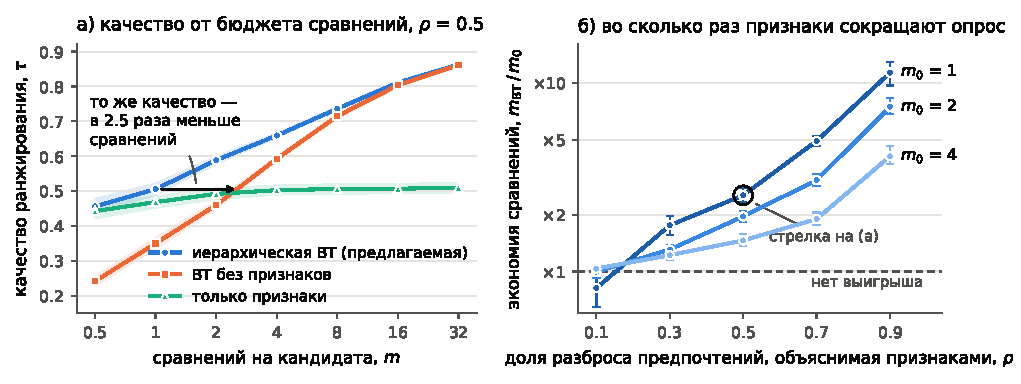
\includegraphics[width=\linewidth]{../figures/main_figure.pdf}
\caption{(а)~Качество ранжирования~\eqref{eq:tau} в зависимости от бюджета при $\rho=0{,}5$; полосы~--- 95\,\%-е интервалы. Иерархической модели при одном сравнении на объект хватает качества, которого модель без признаков достигает лишь при $m\approx2{,}5$. (б)~Экономия~\eqref{eq:saving} при $m_0\in\{1,2,4\}$: растёт с $\rho$ и убывает с $m_0$; при $\rho=0{,}1$ и $m_0=1$ признаки слегка мешают (оценивание $\theta$ по немногим сравнениям).}
\label{fig:main}
\end{figure}

\paragraph{Г1.}
Экономия растёт с $\rho$ (рис.~\ref{fig:main}): при $m_0=1$ она равна $2{,}54$ $[2{,}32;\,2{,}78]$ при $\rho=0{,}5$, $4{,}93$ $[4{,}62;\,5{,}24]$ при $\rho=0{,}7$ и $11{,}4$ $[9{,}7;\,12{,}9]$ при $\rho=0{,}9$. При $\rho=0{,}1$ и $m_0=1$ экономия $0{,}82$ $[0{,}65;\,1{,}00]$: почти бесполезные признаки при очень малом опросе немного вредят, потому что $\theta$ оценивается по тем же немногим сравнениям. С ростом $m_0$ экономия падает: при большом опросе модель без признаков догоняет иерархическую.

\begin{figure}[t]
\centering
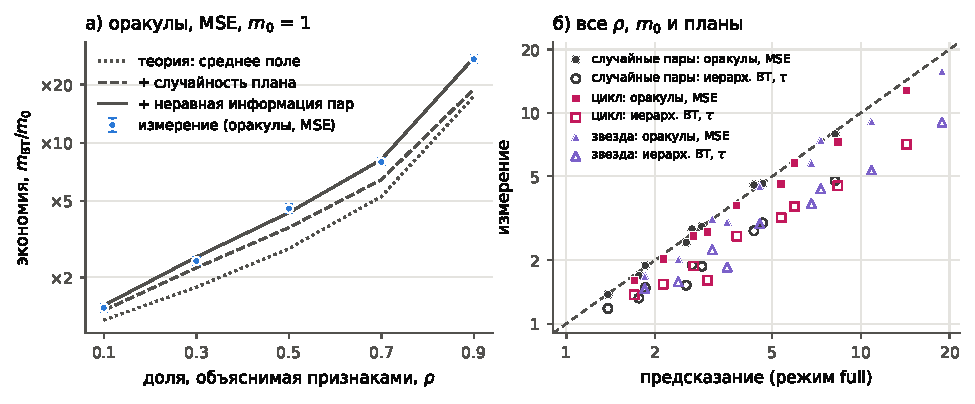
\includegraphics[width=\linewidth]{../figures/fig_theory_check.pdf}
\caption{(а)~Экономия оракула по MSE при $m_0=1$: среднее поле~\eqref{eq:closed} (точки), учёт случайности плана (штрих) и неравной информации пар (сплошная линия) против измерения. (б)~Полный прогноз против измерения для всех $\rho$, $m_0$ и планов; закрашенные маркеры~--- оракулы по MSE, полые~--- иерархическая модель по $\tau$.}
\label{fig:theory}
\end{figure}

\begin{table}[t]
\caption{Экономия $\kappa(m_0)$~\eqref{eq:saving} при случайных парах: три прогноза до эксперимента и измерения (в скобках 95\,\%-е интервалы). <<Откл.>>~--- отклонение измерения оракула от полного прогноза. Полный прогноз точен в пределах 5\,\% во всех ячейках; экономия иерархической модели по $\tau$ ниже из-за оценивания $\theta,\lambda$ и насыщения рангового критерия.}
\label{tab:theory}
\centering\scriptsize
\begin{tabular}{cc ccc cc c}
\toprule
& & \multicolumn{3}{c}{прогноз до эксперимента} & \multicolumn{2}{c}{оракулы, MSE} & иерарх.\ BT, $\tau$ \\
\cmidrule(lr){3-5}\cmidrule(lr){6-7}\cmidrule(lr){8-8}
$\rho$ & $m_0$ & ср.\ поле \eqref{eq:closed} & + план & + инф.\ пар & измерение & откл. & измерение \\
\midrule
0{,}1 & 1 & 1{,}20 & 1{,}35 & 1{,}43 & 1{,}39 \scriptsize[1{,}33; 1{,}46] & $-3$\% & 0{,}87 \scriptsize[0{,}77; 0{,}98] \\
0{,}1 & 2 & 1{,}10 & 1{,}16 & 1{,}21 & 1{,}21 \scriptsize[1{,}18; 1{,}24] & $+0$\% & 1{,}01 \scriptsize[0{,}95; 1{,}06] \\
0{,}1 & 4 & 1{,}05 & 1{,}07 & 1{,}10 & 1{,}12 \scriptsize[1{,}10; 1{,}14] & $+2$\% & 1{,}05 \scriptsize[1{,}01; 1{,}09] \\
0{,}3 & 1 & 1{,}78 & 2{,}24 & 2{,}55 & 2{,}43 \scriptsize[2{,}31; 2{,}55] & $-5$\% & 1{,}52 \scriptsize[1{,}36; 1{,}71] \\
0{,}3 & 2 & 1{,}39 & 1{,}58 & 1{,}76 & 1{,}69 \scriptsize[1{,}62; 1{,}77] & $-4$\% & 1{,}32 \scriptsize[1{,}22; 1{,}43] \\
0{,}3 & 4 & 1{,}20 & 1{,}27 & 1{,}38 & 1{,}37 \scriptsize[1{,}34; 1{,}41] & $-1$\% & 1{,}18 \scriptsize[1{,}13; 1{,}22] \\
0{,}5 & 1 & 2{,}82 & 3{,}63 & 4{,}34 & 4{,}55 \scriptsize[4{,}30; 4{,}82] & $+5$\% & 2{,}76 \scriptsize[2{,}54; 2{,}99] \\
0{,}5 & 2 & 1{,}91 & 2{,}26 & 2{,}67 & 2{,}81 \scriptsize[2{,}69; 2{,}93] & $+5$\% & 1{,}90 \scriptsize[1{,}78; 2{,}05] \\
0{,}5 & 4 & 1{,}46 & 1{,}59 & 1{,}85 & 1{,}89 \scriptsize[1{,}83; 1{,}96] & $+2$\% & 1{,}48 \scriptsize[1{,}40; 1{,}57] \\
0{,}7 & 1 & 5{,}25 & 6{,}43 & 8{,}17 & 7{,}94 \scriptsize[7{,}68; 8{,}31] & $-3$\% & 4{,}76 \scriptsize[4{,}36; 5{,}16] \\
0{,}7 & 2 & 3{,}13 & 3{,}65 & 4{,}64 & 4{,}62 \scriptsize[4{,}40; 4{,}85] & $-0$\% & 3{,}01 \scriptsize[2{,}80; 3{,}21] \\
0{,}7 & 4 & 2{,}06 & 2{,}28 & 2{,}89 & 2{,}89 \scriptsize[2{,}78; 3{,}01] & $+0$\% & 1{,}87 \scriptsize[1{,}78; 1{,}98] \\
0{,}9 & 1 & 17{,}40 & 18{,}97 & 27{,}56 & 27{,}11 \scriptsize[25{,}74; 28{,}36] & $-2$\% & 11{,}77 \scriptsize[10{,}59; 12{,}96] \\
0{,}9 & 2 & 9{,}20 & 9{,}95 & 14{,}49 & 14{,}12 \scriptsize[13{,}50; 14{,}71] & $-3$\% & 6{,}94 \scriptsize[6{,}42; 7{,}43] \\
0{,}9 & 4 & 5{,}10 & 5{,}44 & 7{,}96 & 7{,}67 \scriptsize[7{,}36; 7{,}96] & $-4$\% & 3{,}87 \scriptsize[3{,}64; 4{,}22] \\
\bottomrule
\end{tabular}

\end{table}

\paragraph{Г2.}
Среднее поле~\eqref{eq:closed} систематически занижает экономию оракула по MSE~--- до 1,6 раза при $\rho=0{,}9$, как и следует из теоремы~\ref{thm:jensen}. Учёт случайности плана увеличивает прогноз в 1,02--1,29 раза (сильнее при малом $m_0$), учёт неравной информации пар~--- ещё в 1,03--1,46 раза (сильнее при большом $\rho$, когда разности полезностей велики). После обоих поправок отклонение измерения от прогноза лежит в пределах $\pm5\,\%$ во всех 15 ячейках (табл.~\ref{tab:theory}, рис.~\ref{fig:theory}), т.\,е.\ лапласово приближение при случайных парах точно, а расхождение среднего поля объясняется двумя эффектами внутри модели. Переход от оракула к иерархической модели уменьшает экономию по MSE в 0,52--0,98 раза (сильнее всего при $\rho=0{,}9$ и $m_0=1$, когда $\theta$ и $\lambda$ оцениваются по немногим сравнениям), переход от MSE к $\tau$~--- ещё в 0,59--0,96 раза. Поэтому прогноз по MSE служит для $\tau$ оценкой сверху; это наблюдение эксперимента, а не доказанное утверждение.

\begin{figure}[t]
\centering
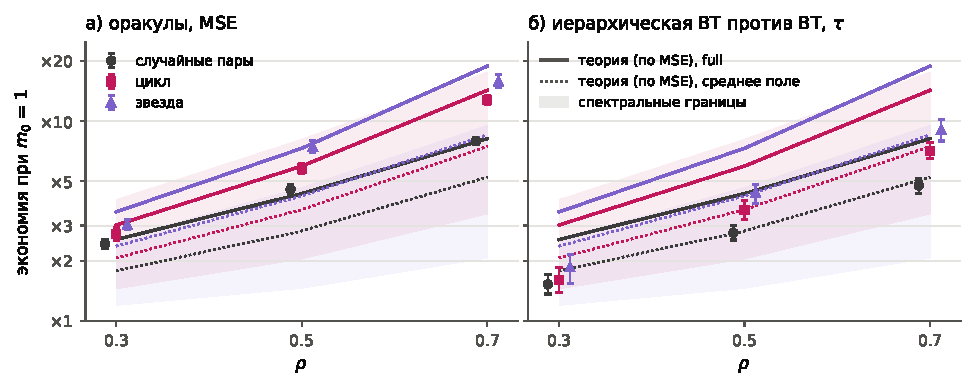
\includegraphics[width=\linewidth]{../figures/fig_designs.pdf}
\caption{Экономия при $m_0=1$ для трёх планов опроса: случайные пары, цикл (каждый объект сравнивается с двумя соседями), звезда (все объекты сравниваются с одним). (а)~Оракулы по MSE; (б)~иерархическая модель по $\tau$. Линии~--- прогнозы (сплошная~--- полный, пунктир~--- среднее поле), полосы~--- спектральные границы~\eqref{eq:bounds}.}
\label{fig:designs}
\end{figure}

\begin{table}[t]
\caption{Экономия при $m_0=1$ для разных планов опроса. Разреженные планы дают большую экономию; полный прогноз на них завышает измерение до 16\,\%.}
\label{tab:designs}
\centering\scriptsize
\begin{tabular}{lc c cc cc}
\toprule
план & $\rho$ & границы \eqref{eq:bounds} & ср.\ поле & full & оракулы, MSE & иерарх.\ BT, $\tau$ \\
\midrule
случайные пары & 0{,}3 & [1{,}78; 1{,}78] & 1{,}78 & 2{,}55 & 2{,}43 \scriptsize[2{,}31; 2{,}55] & 1{,}52 \scriptsize[1{,}36; 1{,}71] \\
случайные пары & 0{,}5 & [2{,}82; 2{,}82] & 2{,}82 & 4{,}34 & 4{,}55 \scriptsize[4{,}30; 4{,}82] & 2{,}76 \scriptsize[2{,}54; 2{,}99] \\
случайные пары & 0{,}7 & [5{,}25; 5{,}25] & 5{,}25 & 8{,}17 & 7{,}94 \scriptsize[7{,}68; 8{,}31] & 4{,}76 \scriptsize[4{,}36; 5{,}16] \\
цикл & 0{,}3 & [1{,}45; 4{,}05] & 2{,}07 & 3{,}02 & 2{,}72 \scriptsize[2{,}53; 2{,}92] & 1{,}61 \scriptsize[1{,}39; 1{,}85] \\
цикл & 0{,}5 & [2{,}04; 8{,}11] & 3{,}61 & 5{,}96 & 5{,}79 \scriptsize[5{,}49; 6{,}12] & 3{,}60 \scriptsize[3{,}23; 3{,}99] \\
цикл & 0{,}7 & [3{,}43; 17{,}60] & 7{,}47 & 14{,}28 & 12{,}79 \scriptsize[12{,}17; 13{,}46] & 7{,}10 \scriptsize[6{,}52; 7{,}80] \\
звезда & 0{,}3 & [1{,}20; 2{,}56] & 2{,}37 & 3{,}51 & 3{,}03 \scriptsize[2{,}86; 3{,}22] & 1{,}86 \scriptsize[1{,}54; 2{,}16] \\
звезда & 0{,}5 & [1{,}46; 4{,}65] & 4{,}23 & 7{,}31 & 7{,}43 \scriptsize[6{,}94; 7{,}98] & 4{,}37 \scriptsize[3{,}86; 4{,}82] \\
звезда & 0{,}7 & [2{,}06; 9{,}51] & 8{,}55 & 18{,}86 & 15{,}77 \scriptsize[14{,}80; 17{,}06] & 9{,}05 \scriptsize[7{,}96; 10{,}25] \\
\bottomrule
\end{tabular}

\end{table}

\paragraph{Г3.}
На разреженных планах экономия больше, чем на случайных, при всех $\rho$, $m_0$ и критериях (рис.~\ref{fig:designs}, табл.~\ref{tab:designs}). При $\rho=0{,}7$, $m_0=1$ экономия оракула по MSE равна 7,9 для случайных пар, 12,8 для цикла и 15,8 для звезды; у иерархической модели по $\tau$~--- 4,8, 7,1 и 9,1. Решение среднего поля лежит внутри границ~\eqref{eq:bounds}, однако измерение часто их превышает: границы выведены для среднего поля, а эффекты плана и информации пар выводят за них. Полный прогноз на цикле завышает экономию на 3--14\,\%, на звезде~--- до 16\,\% при $\rho=0{,}3$ и $0{,}7$ (при $\rho=0{,}5$ совпадает с измерением); вероятная причина~--- неточность лапласова приближения для контрастов, которые план определяет слабо (длинные пути по циклу, сравнения только через центр звезды).

\subsection{Реальные данные: оценки сложности слов}
\label{sec:real}

Прямых данных о предпочтениях носителей татарского языка между заменами заимствований нет. Поэтому гипотеза Г4 проверяется на открытых данных с той же структурой: для английского слова в контексте собраны кандидаты на замену (набор BenchLS~\citep{paetzold2016benchmarking} в версии из~\citep{qiang2020lexical}), а сложность слов независимо оценили 11 человек, изучающих английский как иностранный, по шкале от 1 до 6 (Word Complexity Lexicon~\citep{maddela2018word}). Группа~--- целевое слово вместе с заменами, объект~--- слово, предпочтение~--- выбор более простого слова. Каждый аннотатор, оценивший оба слова пары по-разному, даёт одно сравнение; пары с равными оценками отбрасываются. Оставлены группы, где не меньше четырёх слов есть в словаре: 721 группа, 2641 различное слово, 74\,477 сравнений (55\,656 ничьих отброшено). Одно слово может входить в несколько групп, поэтому граф сравнений не распадается на блоки~--- это случай пересекающихся групп из~\eqref{eq:spectral}.

Признаки: частота слова в логарифмической шкале Ципфа, длина, число слогов и средний логарифм вероятности символа по символьной триграммной модели, обученной на 50 тыс.\ частых английских слов без слов набора (аналог <<правдоподобия формы для языка>>, который для татарского предполагается считать по корпусу). Протокол: 10 случайных разбиений аннотаторов на группы A (6 человек) и B (5 человек); модели обучаются на подвыборке сравнений группы A, $\lambda$ выбирается по сравнениям одного отложенного аннотатора из A, эталон~--- средняя оценка группы B, контрольные сравнения~--- сравнения группы B. Согласие групп A и B между собой ($\tau$ средних оценок) равно $0{,}566\pm0{,}044$; модель <<только признаки>> достигает $\tau=0{,}565$ уже при $m=0{,}5$, т.\,е.\ признаки объясняют почти всё, что воспроизводится между группами аннотаторов. Чтобы экономию можно было измерить без цензурирования, эксперимент повторяется для подсказок разной силы~--- отдельных признаков и их сочетаний.

\todo{Результаты по реальным данным будут вписаны после пересчёта с выбором $\lambda$ по аннотаторам: $\hat\rho$ для каждого набора признаков, измеренная и предсказанная экономия (рис.\ fig\_real\_theory), кривые качества (рис.\ fig\_real).}

% После пересчёта раскомментировать:
% \begin{figure}[t]
% \centering
% 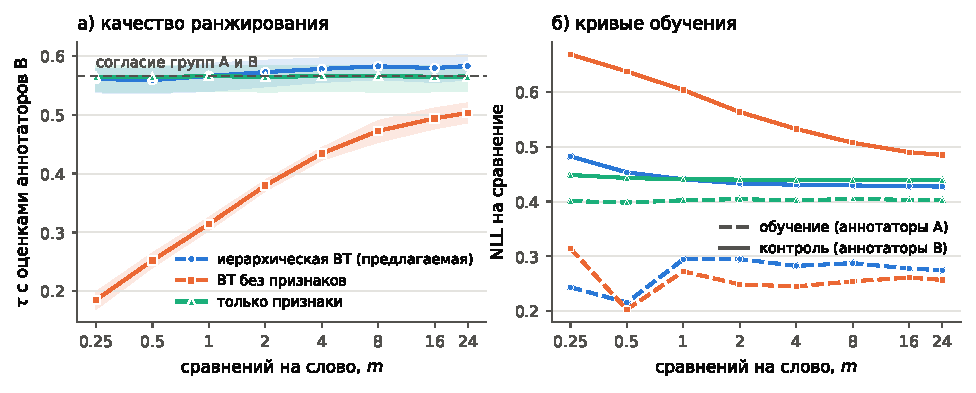
\includegraphics[width=\linewidth]{../figures/fig_real.pdf}
% \caption{...}
% \label{fig:real}
% \end{figure}

\subsection{Анализ ошибки}

\paragraph{Ошибка от объёма выборки.}
Кривые качества и правдоподобия от бюджета (рис.~\ref{fig:main}\,а и \todo{рис.\ fig\_real\,б}) монотонны для модели без признаков; иерархическая модель выходит на плато раньше, модель <<только признаки>> не улучшается с ростом $m$, так как не использует сравнения конкретного объекта. \todo{Обучение против контроля на реальных данных: вписать после пересчёта.}

\paragraph{Ошибка от сложности модели.}
На реальных данных почти весь эффект признаков дают первые два~--- частота и длина; число слогов и символьная модель почти ничего не добавляют (рис.~\ref{fig:complexity}). Зависимость от параметра регуляризации $\lambda$ \todo{описать после пересчёта: оптимум по контролю и выбор по отложенному аннотатору}.

\begin{figure}[t]
\centering
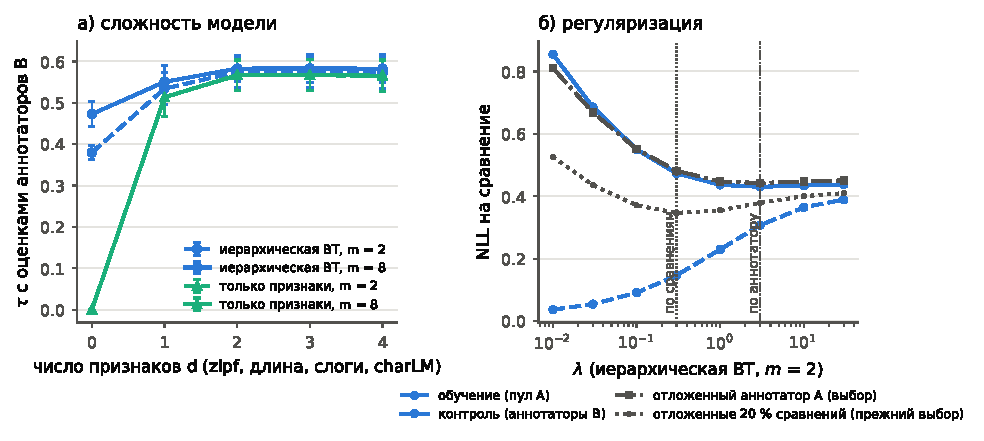
\includegraphics[width=\linewidth]{../figures/fig_complexity.pdf}
\caption{Реальные данные: (а)~качество в зависимости от числа признаков $d$ при $m=2$ и $m=8$; (б)~правдоподобие на обучении и контроле в зависимости от $\lambda$. \todo{подпись обновить после пересчёта}}
\label{fig:complexity}
\end{figure}

\paragraph{Разброс и вычислительная сложность.}
Разброс по повторам показан доверительными полосами на рисунках и стандартными отклонениями в табл.~\ref{tab:models}. Время обучения иерархической модели с выбором $\lambda$ растёт сублинейно в исследованном диапазоне ($N\le1280$, наклон в двойном логарифмическом масштабе 0,75) и при $N=1280$ составляет 0,41~с; прогноз по алгоритму~\ref{alg:mc} при 200 реализациях занимает около 15~с.

\begin{table}[t]
\caption{Сравнение моделей на синтетических и реальных данных при бюджете $m$: качество~\eqref{eq:tau}, доля верно найденных лучших объектов (top-1) и отрицательное логарифмическое правдоподобие контрольных сравнений (среднее $\pm$ стандартное отклонение по повторам). Жирным выделен лучший результат в срезе.}
\label{tab:models}
\centering\scriptsize
\begin{tabular}{lccc}
\toprule
Метод & $\tau$ & top-1 & NLL (контроль) \\
\midrule
\multicolumn{4}{l}{\textit{синтетика, $\rho$ = 0.3, m = 2}} \\
BT без признаков & 0.456 $\pm$ 0.029 & 0.398 $\pm$ 0.091 & 0.606 $\pm$ 0.018 \\
только признаки & 0.369 $\pm$ 0.048 & 0.351 $\pm$ 0.078 & 0.624 $\pm$ 0.016 \\
иерархическая BT & 0.511 $\pm$ 0.033 & 0.450 $\pm$ 0.093 & 0.574 $\pm$ 0.017 \\
BT, $\lambda = 1/V$ & 0.459 $\pm$ 0.030 & 0.404 $\pm$ 0.089 & 0.599 $\pm$ 0.016 \\
оракул (известное $\mu$) & \textbf{0.531} $\pm$ 0.031 & \textbf{0.485} $\pm$ 0.088 & \textbf{0.570} $\pm$ 0.017 \\
\midrule
\multicolumn{4}{l}{\textit{синтетика, $\rho$ = 0.5, m = 2}} \\
BT без признаков & 0.460 $\pm$ 0.030 & 0.349 $\pm$ 0.084 & 0.596 $\pm$ 0.015 \\
только признаки & 0.492 $\pm$ 0.041 & 0.446 $\pm$ 0.060 & 0.571 $\pm$ 0.016 \\
иерархическая BT & 0.589 $\pm$ 0.031 & 0.522 $\pm$ 0.076 & 0.536 $\pm$ 0.020 \\
BT, $\lambda = 1/V$ & 0.461 $\pm$ 0.030 & 0.352 $\pm$ 0.081 & 0.597 $\pm$ 0.018 \\
оракул (известное $\mu$) & \textbf{0.604} $\pm$ 0.030 & \textbf{0.526} $\pm$ 0.075 & \textbf{0.535} $\pm$ 0.025 \\
\midrule
\multicolumn{4}{l}{\textit{синтетика, $\rho$ = 0.7, m = 2}} \\
BT без признаков & 0.456 $\pm$ 0.028 & 0.398 $\pm$ 0.053 & 0.596 $\pm$ 0.014 \\
только признаки & 0.626 $\pm$ 0.030 & 0.572 $\pm$ 0.072 & 0.501 $\pm$ 0.015 \\
иерархическая BT & 0.672 $\pm$ 0.028 & 0.607 $\pm$ 0.065 & 0.484 $\pm$ 0.020 \\
BT, $\lambda = 1/V$ & 0.456 $\pm$ 0.028 & 0.393 $\pm$ 0.053 & 0.599 $\pm$ 0.016 \\
оракул (известное $\mu$) & \textbf{0.685} $\pm$ 0.022 & \textbf{0.614} $\pm$ 0.060 & \textbf{0.481} $\pm$ 0.018 \\
\midrule
\multicolumn{4}{l}{\textit{реальные данные, m = 2}} \\
BT без признаков & 0.380 $\pm$ 0.017 & 0.522 $\pm$ 0.033 & 0.564 $\pm$ 0.010 \\
только признаки & 0.565 $\pm$ 0.037 & 0.669 $\pm$ 0.042 & 0.440 $\pm$ 0.041 \\
иерархическая BT & \textbf{0.573} $\pm$ 0.038 & \textbf{0.685} $\pm$ 0.034 & \textbf{0.433} $\pm$ 0.041 \\
\midrule
\multicolumn{4}{l}{\textit{реальные данные, m = 8}} \\
BT без признаков & 0.473 $\pm$ 0.031 & 0.587 $\pm$ 0.036 & 0.508 $\pm$ 0.025 \\
только признаки & 0.566 $\pm$ 0.038 & 0.669 $\pm$ 0.045 & 0.439 $\pm$ 0.039 \\
иерархическая BT & \textbf{0.583} $\pm$ 0.033 & \textbf{0.691} $\pm$ 0.036 & \textbf{0.429} $\pm$ 0.043 \\
\bottomrule
\end{tabular}

\end{table}

%=====================================================================
\section{Заключение}

Получен априорный прогноз того, сколько попарных сравнений заменяют признаки объектов в иерархической модели Брэдли--Терри. Замкнутая формула~\eqref{eq:closed} выражает экономию через долю $\rho$ дисперсии предпочтений, объясняемую признаками, и даёт главную зависимость $\rho/(1-\rho)$; для произвольного плана доказаны спектральные границы, из которых следует, что признаки ценнее всего при разреженном опросе. Формула среднего поля даёт нижнюю оценку ожидаемого риска, а уточнённый прогноз методом Монте-Карло совпадает с экспериментом в пределах 5\,\% при случайном выборе пар. Измерения показывают, какую часть выигрыша съедает оценивание параметров и переход к ранговому критерию. \todo{Итог по реальным данным.}

Прогноз позволяет до опроса оценить, сколько ответов носителей понадобится для ранжирования замен заимствований, и выбрать план опроса. Дальнейшая работа: применение к татарским заменам с признаками по корпусу и оценками языковой модели в роли подсказки, уточнение прогноза для разреженных планов и прогноз для критерия поиска лучшего объекта, а не полного порядка.

\bibliographystyle{unsrtnat}
\bibliography{references}

\end{document}
